\documentclass[10pt]{article}
\usepackage[utf8]{inputenc}
\usepackage[T1]{fontenc}
\usepackage{graphicx}
\usepackage[export]{adjustbox}
\graphicspath{ {./images/} }
\usepackage{amsmath}
\usepackage{amsfonts}
\usepackage{amssymb}
\usepackage[version=4]{mhchem}
\usepackage{stmaryrd}
\usepackage{mathrsfs}
\usepackage{bbold}

\title{Generalization, Model Selection, and Validation }


\author{Machine Learning Course - CS-433\\
Oct 10, 2023\\
Nicolas Flammarion}
\date{}


\begin{document}
\maketitle
EPFL

\section*{Generalization, validation?}
\begin{center}
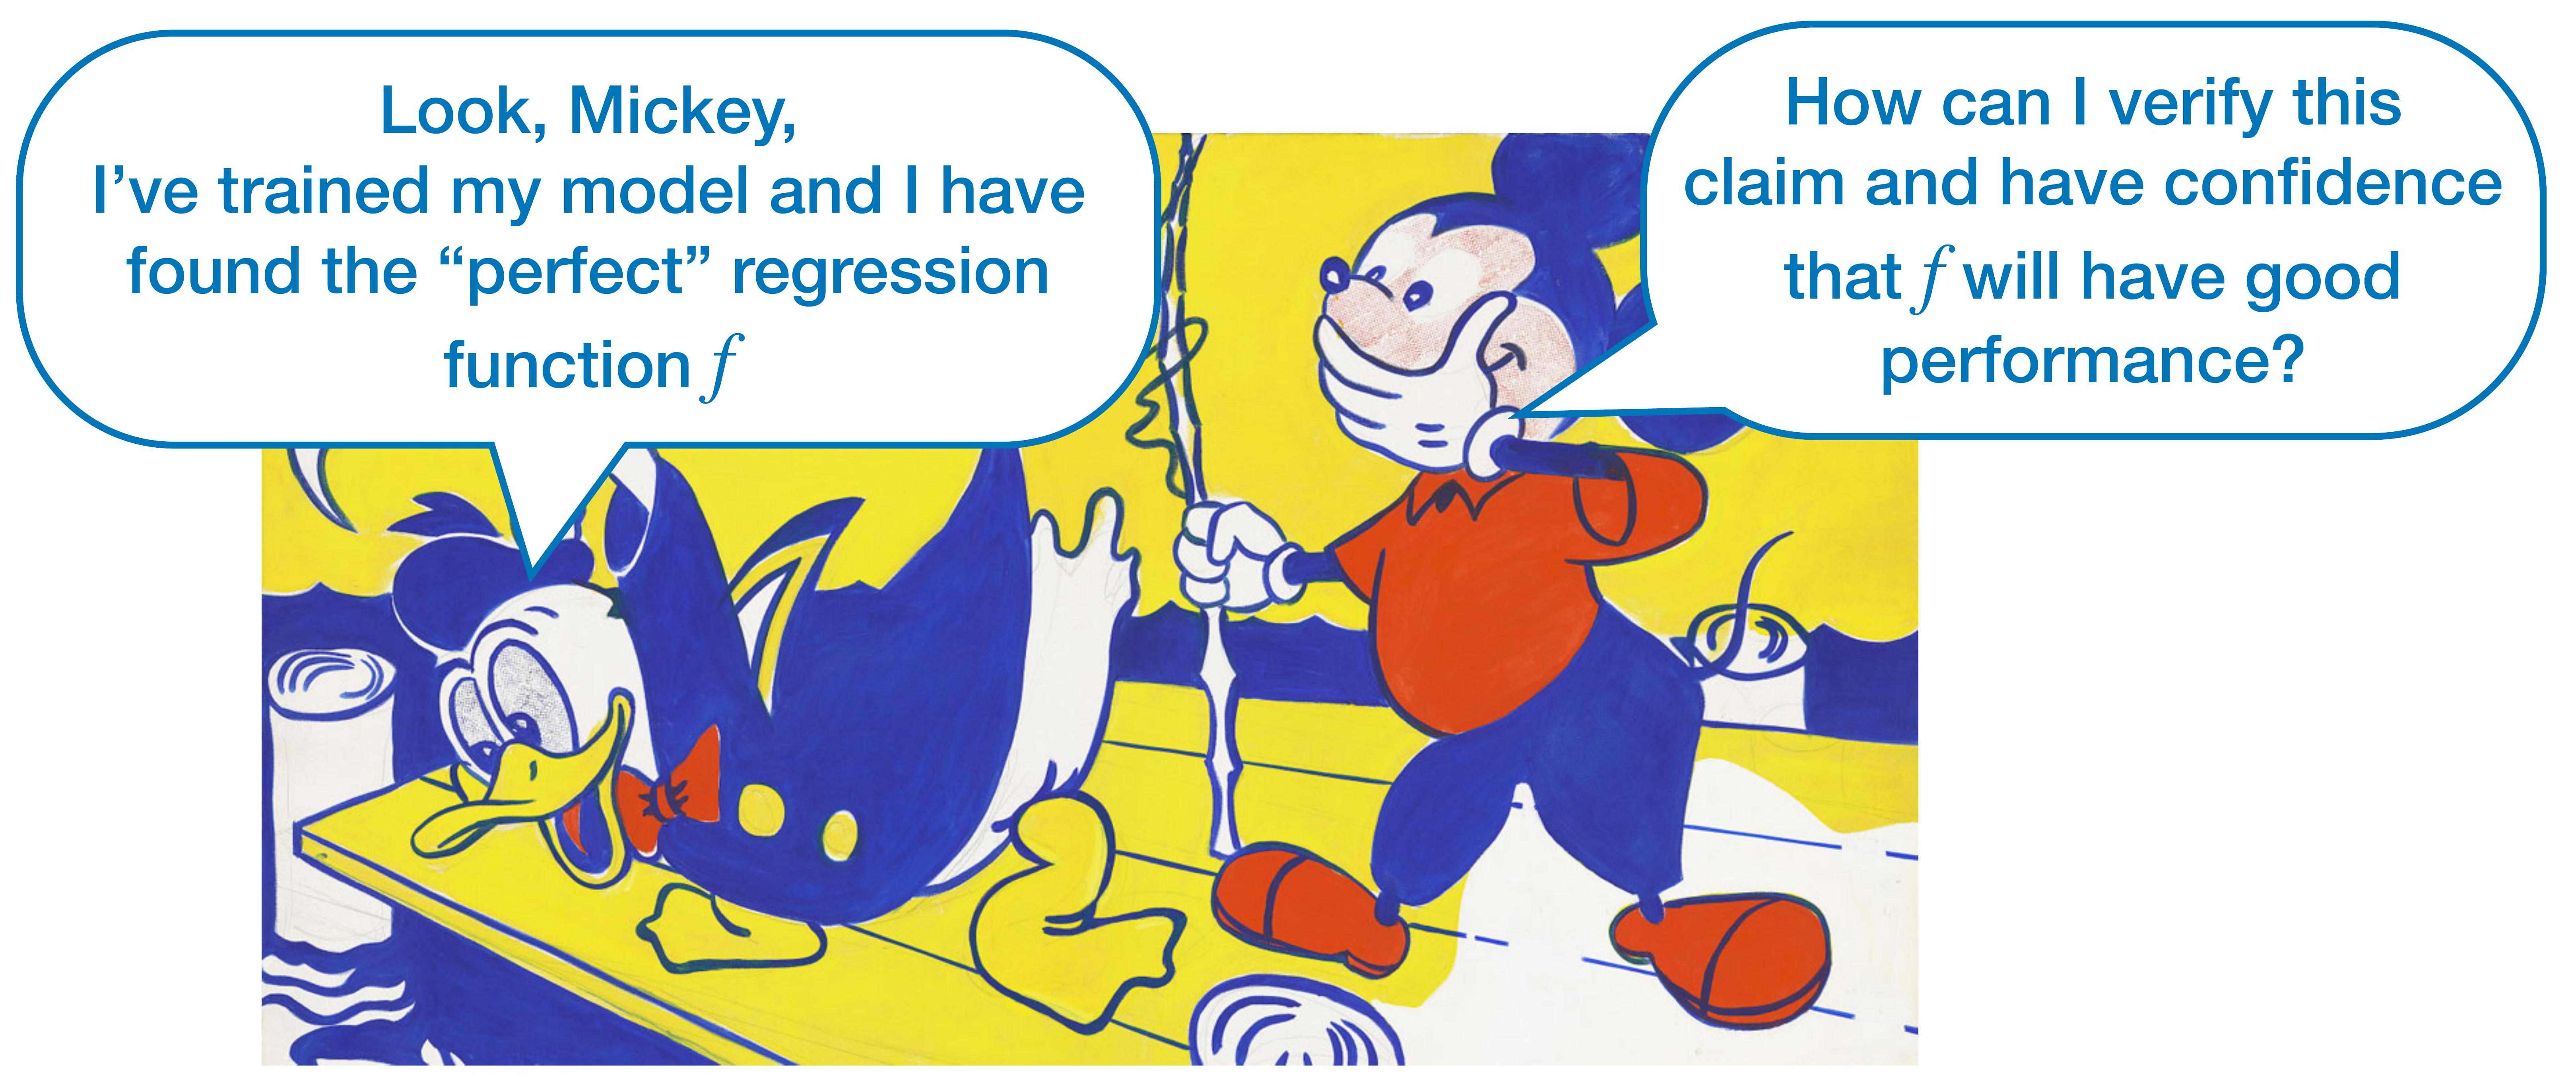
\includegraphics[max width=\textwidth]{2023_12_30_b4c98a1755bce7fa9493g-02}
\end{center}

\section*{What is the model selection problem?}
\begin{itemize}
  \item Ridge regression: $w_{\lambda}=\arg \min _{w} \frac{1}{2 N} \sum_{n=1}^{N}\left(y_{n}-x_{n}^{\top} w\right)^{2}+\lambda\|w\|_{2}^{2}$
  \item $\lambda$ can be tuned to control the model complexity (to reduce overfitting)
\end{itemize}

Hyperparameter

\begin{itemize}
  \item In practice: $\left(\lambda_{1}, \cdots, \lambda_{k}\right) \longrightarrow$ Algorithm $\longrightarrow\left(w_{1}, \cdots, w_{k}\right)$

  \item Which $\lambda$ should we use?

  \item Polynomial feature expansion: ${ }_{\left(x_{(1)}, x_{(2)}\right)} \xrightarrow{\phi} \begin{aligned} & \left(x_{(1)}, x_{(2)}, x_{(1)}^{2}+x_{(2)}^{2}\right) \\ & \left(x_{(1)}, x_{(2)}, 5 x_{(1)}^{2}+2 x_{(2)}^{2}, x_{(2)}^{3}+2 x_{(1)}\right)\end{aligned}$

  \item Enrich the model complexity, by augmenting the feature vector $x$.

  \item Here the degree $d$ is the hyperparameter

\end{itemize}

We are facing the same problem: how do we choose these hyperparameters?

\section*{Model selection for neural networks}
\begin{center}
\begin{tabular}{|l|}
\hline
\multicolumn{1}{|c|}{Algorithms?} \\
SGD \\
Adam \\
Which step-size? \\
Which batch-size? \\
Which momentum? \\
\hline
\end{tabular}
\end{center}

\begin{center}
\begin{tabular}{|l|}
\hline
\multicolumn{1}{|c|}{Architectures?} \\
 \\
FullyConnected \\
ConvNet \\
ResNet \\
Transformer \\
Which width? \\
Which depth? \\
Batch normalization? \\
\hline
\end{tabular}
\end{center}

\begin{center}
\begin{tabular}{|l|}
\hline
\multicolumn{1}{|c|}{Regularizations?} \\
Weight decay? \\
Early stopping? \\
Data augmentations? \\
\hline
\end{tabular}
\end{center}

\section*{Probabilistic Setup}
Data Model:

Unknown distribution $\mathscr{D}$ with range $\mathscr{X} \times \mathscr{Y}$

We see a dataset $S$ of independent samples from $\mathscr{D}$ :

$$
S=\left\{\left(x_{n}, y_{n}\right)\right\}_{n=1}^{N} \sim \mathscr{D} \quad \text { i.i.d. }
$$

Learning Algorithm:

\begin{center}
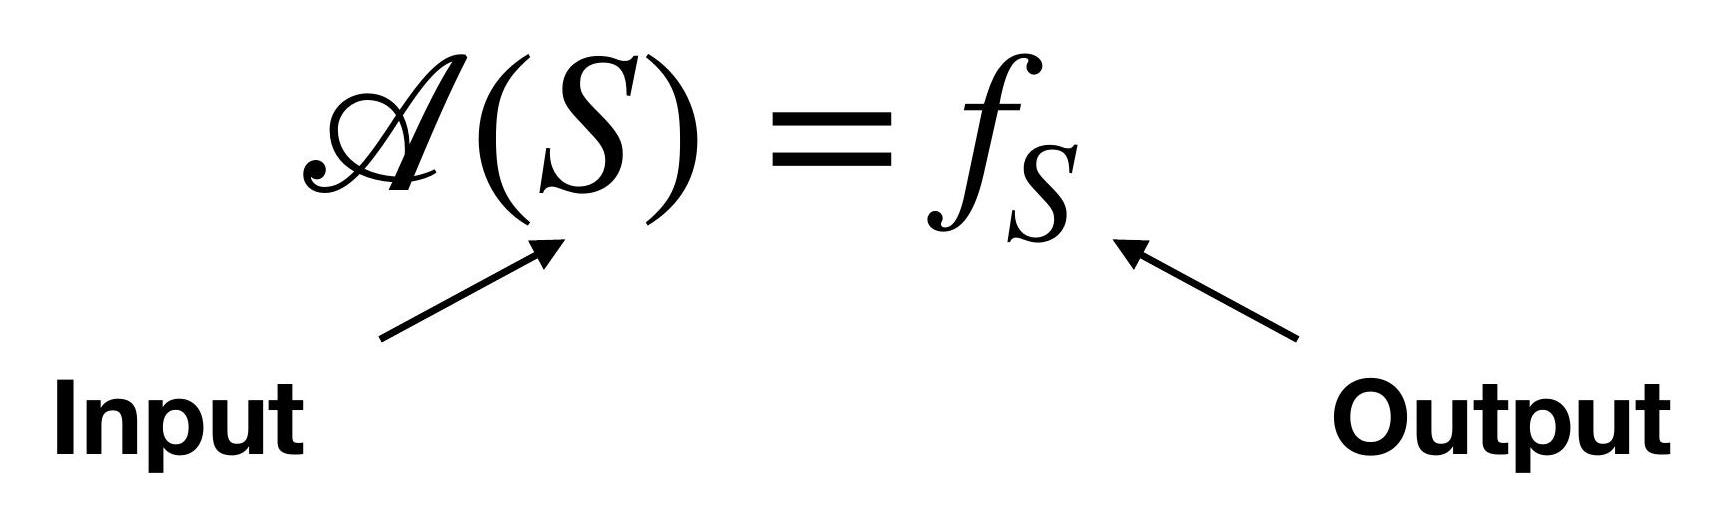
\includegraphics[max width=\textwidth]{2023_12_30_b4c98a1755bce7fa9493g-05}
\end{center}

Ridge regression: gradient descent or least-squares estimator

Can add a subscript $f_{S, \lambda}$ to indicate the model dependency

\section*{Generalization Error: how accurate is $f$ at predicting?}
We compute the expected error over all samples drawn from distribution $\mathscr{D}$ :

$$
L_{\mathscr{D}}(f)=\mathbb{E}_{(x, y) \sim \mathscr{D}}[\ell(y, f(x))]
$$

where $\ell(\cdot, \cdot)$ is the loss function

\begin{itemize}
  \item Ex: $\ell\left(y, y^{\prime}\right)=\frac{1}{2}\left(y-y^{\prime}\right)^{2}$, logistic loss, hinge loss
\end{itemize}

The quantity $L_{\mathscr{D}}(f)$ has many names: $\left\{\begin{array}{l}\text { True } \\ \text { Expected } \\ \text { Generalization }\end{array}\left\{\begin{array}{l}\text { Risk } \\ \text { Error } \\ \text { Loss }\end{array}\right.\right.$

This is the quantity we are fundamentally interested in

\section*{Generalization Error: how accurate is $f$ at predicting?}
We compute the expected error over all samples drawn from distribution $\mathscr{D}$ :

$$
L_{\mathscr{D}}(f)=\mathbb{E}_{(x, y) \sim \mathscr{D}}[\ell(y, f(x))]
$$

where $\ell(\cdot, \cdot)$ is the loss function

\begin{itemize}
  \item Ex: $\ell\left(y, y^{\prime}\right)=\frac{1}{2}\left(y-y^{\prime}\right)^{2}$, logistic loss, hinge loss
\end{itemize}

The quantity $L_{\mathscr{D}}(f)$ has many names: $\left\{\begin{array}{l}\text { True } \\ \text { Expected } \\ \text { Generalization }\end{array}\left\{\begin{array}{l}\text { Risk } \\ \text { Error } \\ \text { Loss }\end{array}\right.\right.$

This is the quantity we are fundamentally interested in

\section*{Empirical Error: what we can compute}
We can approximate the true error by averaging the loss function over the dataset

$$
L_{S}(f)=\frac{1}{|S|} \sum_{\left(x_{n}, y_{n}\right) \in S} \ell\left(y_{n}, f\left(x_{n}\right)\right)
$$

Also called: empirical risk/error/loss

$\Delta$ The samples are random thus $L_{S}(f)$ is a random variable It is an unbiased estimator of the true error

Law of large number: $L_{S}(f) \underset{|S| \rightarrow \infty}{\rightarrow} L_{\mathscr{D}}(f)$ but fluctuations!

Generalization gap: $\left|L_{\mathscr{D}}(f)-L_{S}(f)\right|$

\section*{Training error: what we are minimizing}
$\Delta$ the prediction function $f_{S}$ is itself a function of the data $S$

When the model has been trained on the same data it is applied to, the empirical error is called the training error:

$$
L_{S}\left(f_{S}\right)=\frac{1}{|S|} \sum_{\left(x_{n}, y_{n}\right) \in S} \ell\left(y_{n}, f_{S}\left(x_{n}\right)\right)
$$

This is the objective function you are minimizing to find the predictor It might not be representative of the error we see on "fresh" samples

The reason that $L_{S}\left(f_{S}\right)$ might not be close to $L_{\mathscr{D}}\left(f_{S}\right)$ is of course overfitting

\section*{Splitting the data}
Problem: Validating model on the same data we trained it on Fix: Split the data into an independent training and test set:

$$
S=S_{\text {train }} \cup S_{\text {test }}
$$

\begin{enumerate}
  \item We learn the function $f_{S_{\text {train }}}$ using the train set

  \item We validate it computing the error on the test set

\end{enumerate}

$$
L_{S_{\text {test }}}\left(f_{S_{\text {train }}}\right)=\frac{1}{\left|S_{\text {test }}\right|} \sum_{\left(y_{n}, x_{n}\right) \in S_{\text {test }}} \ell\left(y_{n}, f_{S_{\text {train }}}\left(x_{n}\right)\right)
$$

$\Rightarrow$ Since $S_{\text {test }}$ and $S_{\text {train }}$ are independent: $L_{S_{\text {test }}}\left(f_{S_{\text {train }}}\right) \approx L_{\mathscr{D}}\left(f_{\text {train }}\right)$

\section*{Splitting the data}
Problem: Validating model on the same data we trained it on

Fix: Split the data into an independent training and test set:

$$
S=S_{\text {train }} \cup S_{\text {test }}
$$

\begin{enumerate}
  \item We learn the function $f_{S_{\text {train }}}$ using the train set

  \item We validate it computing the error on the test set

\end{enumerate}

$$
L_{S_{\text {test }}}\left(f_{S_{\text {train }}}\right)=\frac{1}{\left|S_{\text {test }}\right|} \sum_{\left(y_{n}, x_{n}\right) \in S_{\text {test }}} \ell\left(y_{n}, f_{S_{\text {train }}}\left(x_{n}\right)\right)
$$

$\Rightarrow$ Since $S_{\text {test }}$ and $S_{\text {train }}$ are independent: $L_{S_{\text {test }}}\left(f_{S_{\text {train }}}\right) \approx L_{\mathscr{D}}\left(f_{S_{\text {train }}}\right)$

$\Delta$ We have less data both for the learning and the validation tasks (tradeoff)

\section*{Generalization gap: How far is the test from the true error?}
Claim: given a model $f$ and a test set $S_{\text {test }} \sim \mathscr{D}$ i.i.d. (not used to learn $f$ ) and a loss $\ell(\cdot, \cdot) \in[a, b]$ :

$$
\mathbb{P}\left[|\underbrace{L_{\mathscr{D}}(f)-L_{S_{\text {test }}}(f)}_{\text {Generalization Gap }}| \geq \sqrt{\frac{(b-a)^{2} \ln (2 / \delta)}{2\left|S_{\text {test }}\right|}}\right] \leq \delta
$$

The error decreases as $\mathcal{O}\left(1 / \sqrt{\left|S_{\text {test }}\right|}\right)$ with the number of test points High probability bound: $\delta$ is only in the $\ln$

$\rightarrow$ The more data points we have, the more confident we are that the empirical loss we measure is close to the true loss

\section*{Why do you care?}
\begin{itemize}
  \item Given a predictor $f$ and a dataset $S$ you can control the expected risk:
\end{itemize}

$$
\mathbb{P}(\underbrace{L_{\mathscr{D}}(f)}_{\text {not computable }} \geq \underbrace{L_{S}(f)}_{\text {Computable }}+\underbrace{\sqrt{\frac{(a-b)^{2} \ln (2 / \delta)}{2\left|S_{\text {test }}\right|}}}_{\text {deviation }}) \leq \delta
$$

\begin{itemize}
  \item Given a dataset $S$
\end{itemize}

\begin{enumerate}
  \item Split: $S=S_{\text {train }} \cup S_{\text {test }}$

  \item Train: $\mathscr{A}\left(S_{\text {train }}\right)=f_{S_{\text {train }}}$

  \item Validate:

\end{enumerate}

$$
\mathbb{P}\left(L_{\mathscr{D}}\left(f_{S_{\text {train }}}\right) \geq L_{S_{\text {test }}}\left(f_{S_{\text {train }}}\right)+\sqrt{\frac{(a-b)^{2} \ln (2 / \delta)}{2\left|S_{\text {test }}\right|}}\right) \leq \delta
$$

$\Rightarrow$ We can obtain a probabilistic upper bound on the expected risk

\section*{The proof relies only on concentration inequalities}
Since $\left(x_{n}, y_{n}\right) \in S_{\text {test }}$ are chosen independently, the associated losses $\Theta_{n}=\ell\left(y_{n}, f\left(x_{n}\right)\right) \in[a, b]$ given a fixed $\operatorname{model} f$, are also i.i.d. random variables

Empirical loss: $\frac{1}{N} \sum_{n=1}^{N} \Theta_{n}=\frac{1}{N} \sum_{n=1}^{N} \ell\left(y_{n}, f\left(x_{n}\right)\right)=L_{S_{\text {test }}}(f)$

True loss: $\quad \mathbb{E}\left[\Theta_{n}\right]=\mathbb{E}\left[\ell\left(y_{n}, f\left(x_{n}\right)\right)\right]=L_{\mathscr{D}}(f)$

What is the chance that the empirical loss $L_{S_{\text {test }}}(f)$ deviates from the true loss by more than a given constant?

\begin{itemize}
  \item classically addressed using concentration inequalities
\end{itemize}

\section*{Hoeffding inequality: a simple concentration bound}
Claim: Let $\Theta_{1}, \ldots, \Theta_{N}$ be a sequence of i.i.d. random variables with mean $\mathbb{E}[\Theta]$ and range $[a, b]$

$$
\mathbb{P}\left[\left|\frac{1}{N} \sum_{n=1}^{N} \Theta_{n}-\mathbb{E}[\Theta]\right| \geq \varepsilon\right] \leq 2 e^{-2 N \varepsilon^{2} /(b-a)^{2}} \text { for any } \varepsilon \geq 0
$$

Concentration bound: the empirical mean is concentrated around its mean

A. Use it with $\Theta_{n}=\ell\left(y_{n}, f\left(x_{n}\right)\right)$

B. Equating $\delta=2 e^{-2\left|S_{\text {test }}\right| \varepsilon^{2} /(b-a)^{2}}$ we get $\varepsilon=\sqrt{\frac{(b-a)^{2} \ln (2 / \delta)}{2\left|S_{\text {test }}\right|}} \square$

\section*{Model Selection: pick the best model}
Goal: select the hyperparameters of our model ( $\lambda$ for the ridge regression) We have a set of values $\left\{\lambda_{k}\right\}_{k=1}^{K}$. Which one should we choose?

\begin{enumerate}
  \item Split the data into $S=S_{\text {train }} \cup S_{\text {test }}$, generated independently from $\mathscr{D}$

  \item Run the learning algorithm $K$ times on the same training set $S_{\text {train }}$ to compute the $K$ prediction functions $f_{S_{\text {train }}, \lambda_{k}}$

  \item For each prediction function, compute the test error $L_{S_{\text {test }}}\left(f_{S_{\text {train }}, \lambda_{k}}\right)$

\end{enumerate}

We then choose the value of the parameter $\lambda$ giving the smallest test error

\section*{Examples}
\begin{center}
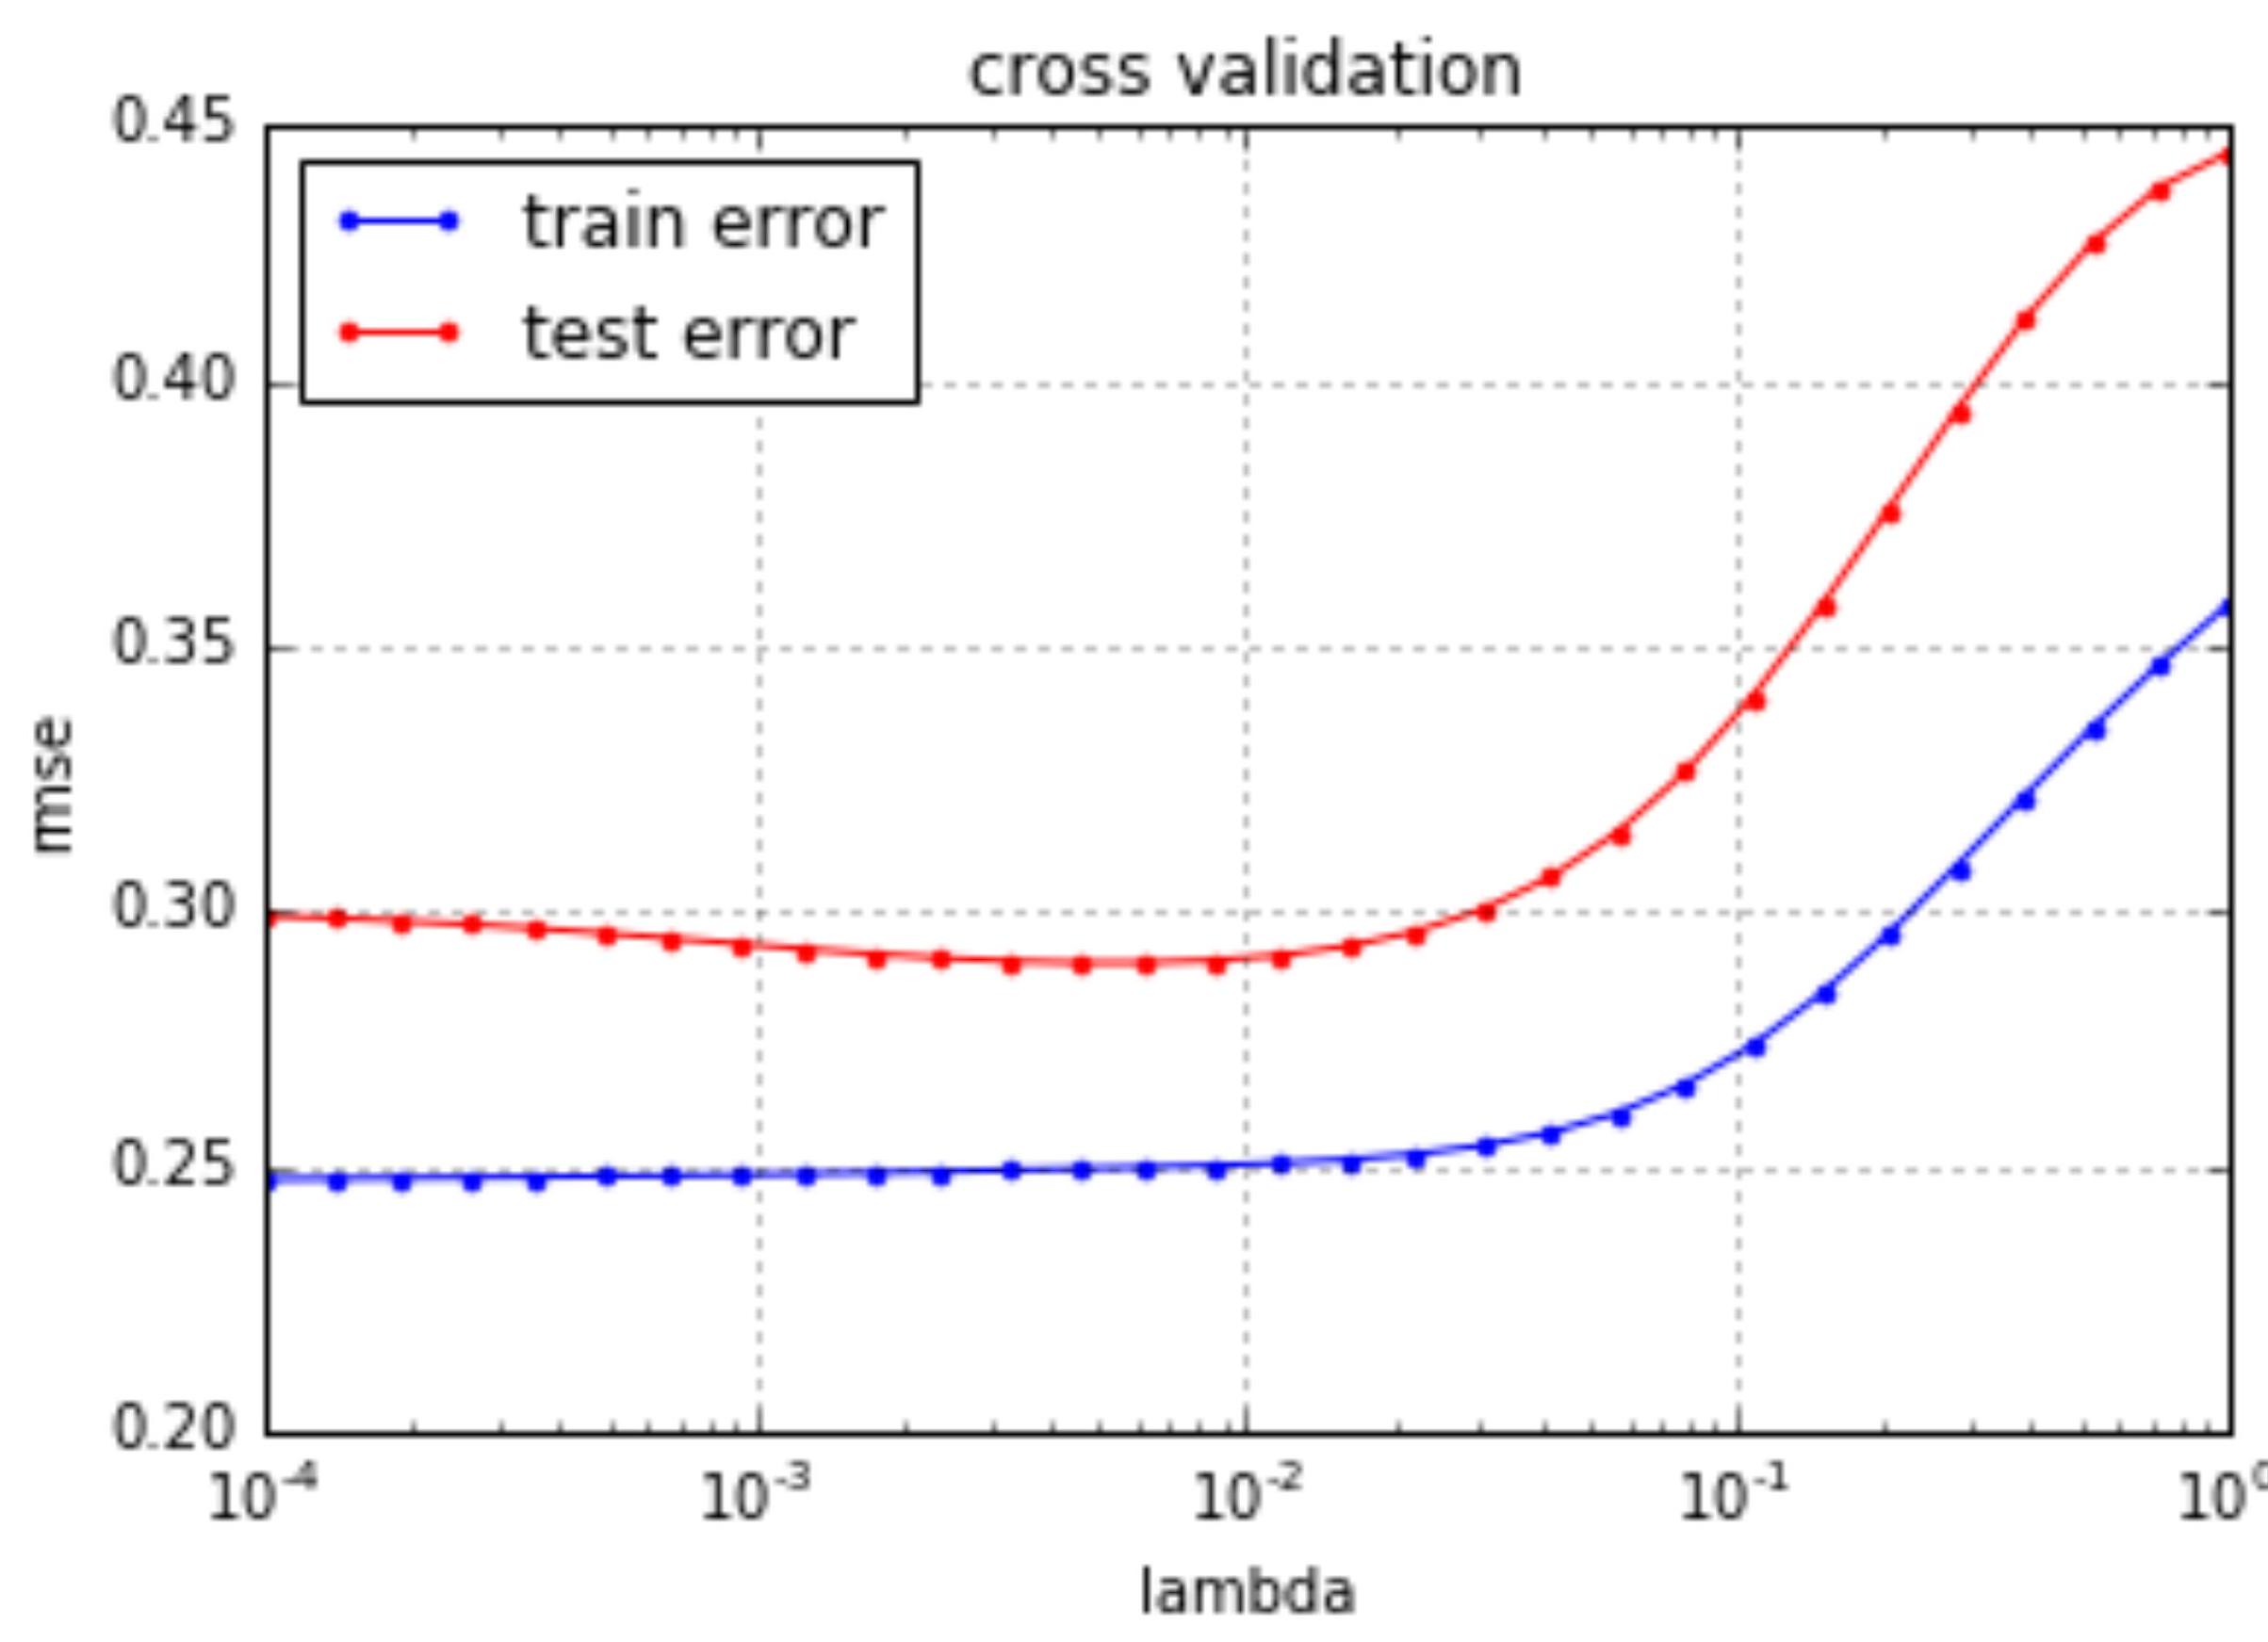
\includegraphics[max width=\textwidth]{2023_12_30_b4c98a1755bce7fa9493g-17}
\end{center}

Ridge regression

\begin{center}
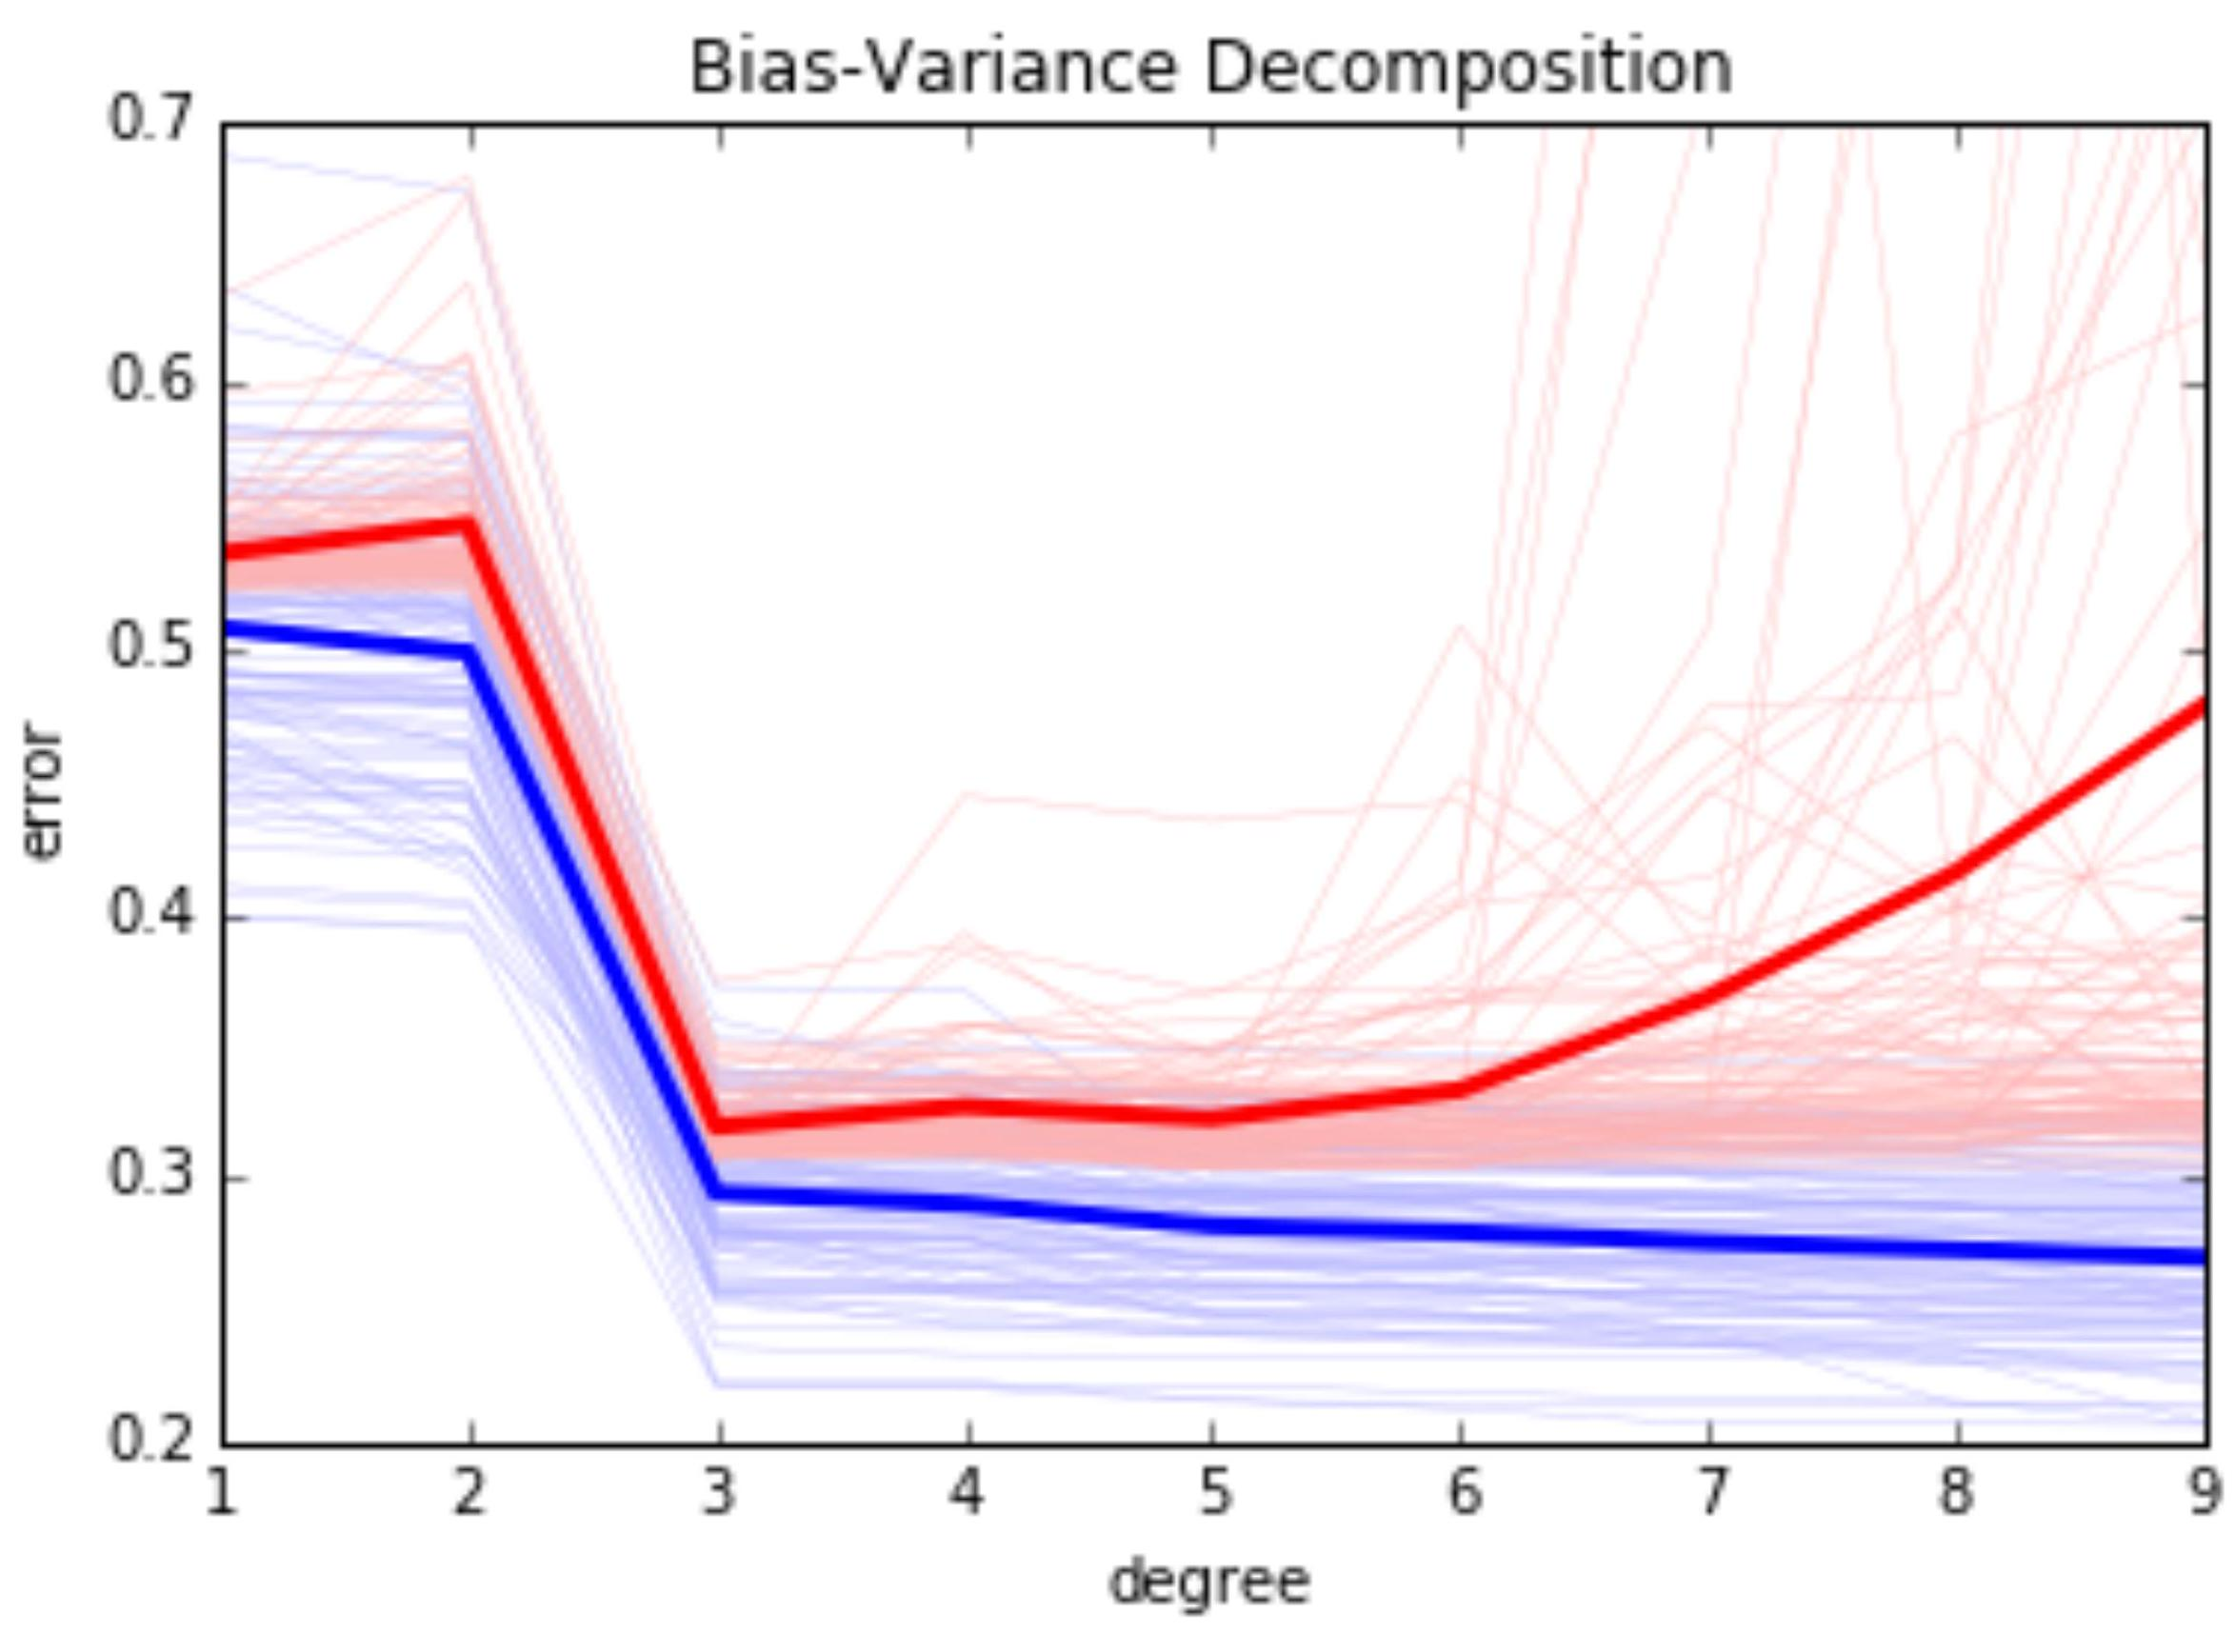
\includegraphics[max width=\textwidth]{2023_12_30_b4c98a1755bce7fa9493g-17(1)}
\end{center}

Degree in case of a polynomial feature expansion

\section*{Does model selection work?}
Two questions:

\begin{itemize}
  \item How do we know that the best function $f_{S_{\operatorname{train}, \lambda}}$ is a good approximation of the best model within our function class?

  \item How do we know that $L_{S_{\text {test }}}\left(f_{S_{\text {train }}, \lambda_{k}}\right) \approx L_{\mathscr{D}}\left(f_{S_{\text {train }}, \lambda_{k}}\right)$ ?

\end{itemize}

We have discussed it for a single model What about several models?

l.e., what is the justification that the min is actually good?

\section*{How far is each of the $K$ test errors $L_{S_{\text {test }}}\left(f_{k}\right)$ from the true $L_{\mathscr{D}}\left(f_{k}\right)$ ?}
Claim: we can bound the maximum deviation for all $K$ candidates, by

$$
\mathbb{P}\left[\max _{k}\left|L_{\mathscr{D}}\left(f_{k}\right)-L_{S_{\text {test }}}\left(f_{k}\right)\right| \geq \sqrt{\frac{(b-a)^{2} \ln (2 K / \delta)}{2\left|S_{\text {test }}\right|}}\right] \leq \delta
$$

\begin{itemize}
  \item The error decreases as $\mathcal{O}\left(1 / \sqrt{\left|S_{\text {test }}\right|}\right)$ with the number test points
  \item When testing $K$ hyper-parameters, the error only goes up by $\sqrt{\ln (K)}$
\end{itemize}

$\Rightarrow$ So we can test many different models without incurring a large penalty

\begin{itemize}
  \item It can be extended to infinitely many models
\end{itemize}

\section*{Proof: A simple union bound}
The proof of this statement follows the proof of the special case $K=1$

$$
\begin{aligned}
\mathbb{P}\left[\max _{k}\left|L_{\mathscr{D}}\left(f_{k}\right)-L_{S_{\text {test }}}\left(f_{k}\right)\right| \geq \varepsilon\right] & =\mathbb{P}\left[\cup_{k}\left\{\left|L_{\mathscr{D}}\left(f_{k}\right)-L_{S_{\text {test }}}\left(f_{k}\right)\right| \geq \varepsilon\right\}\right] \\
& \leq \sum_{k} \mathbb{P}\left[\left|L_{\mathscr{D}}\left(f_{k}\right)-L_{S_{\text {test }}}\left(f_{k}\right)\right| \geq \varepsilon\right] \\
& \leq 2 K e^{-2 N \varepsilon^{2} /(b-a)^{2}}
\end{aligned}
$$

Hence, equating $\delta=2 K e^{-2 N \varepsilon^{2} /(b-a)^{2}}$, we get $\varepsilon=\sqrt{\frac{(b-a)^{2} \ln (2 K / \delta)}{2 N}}$ as stated

If we choose the "best" function according to the empirical risk then its true risk is not too far away from the true risk of the optimal choice

\begin{center}
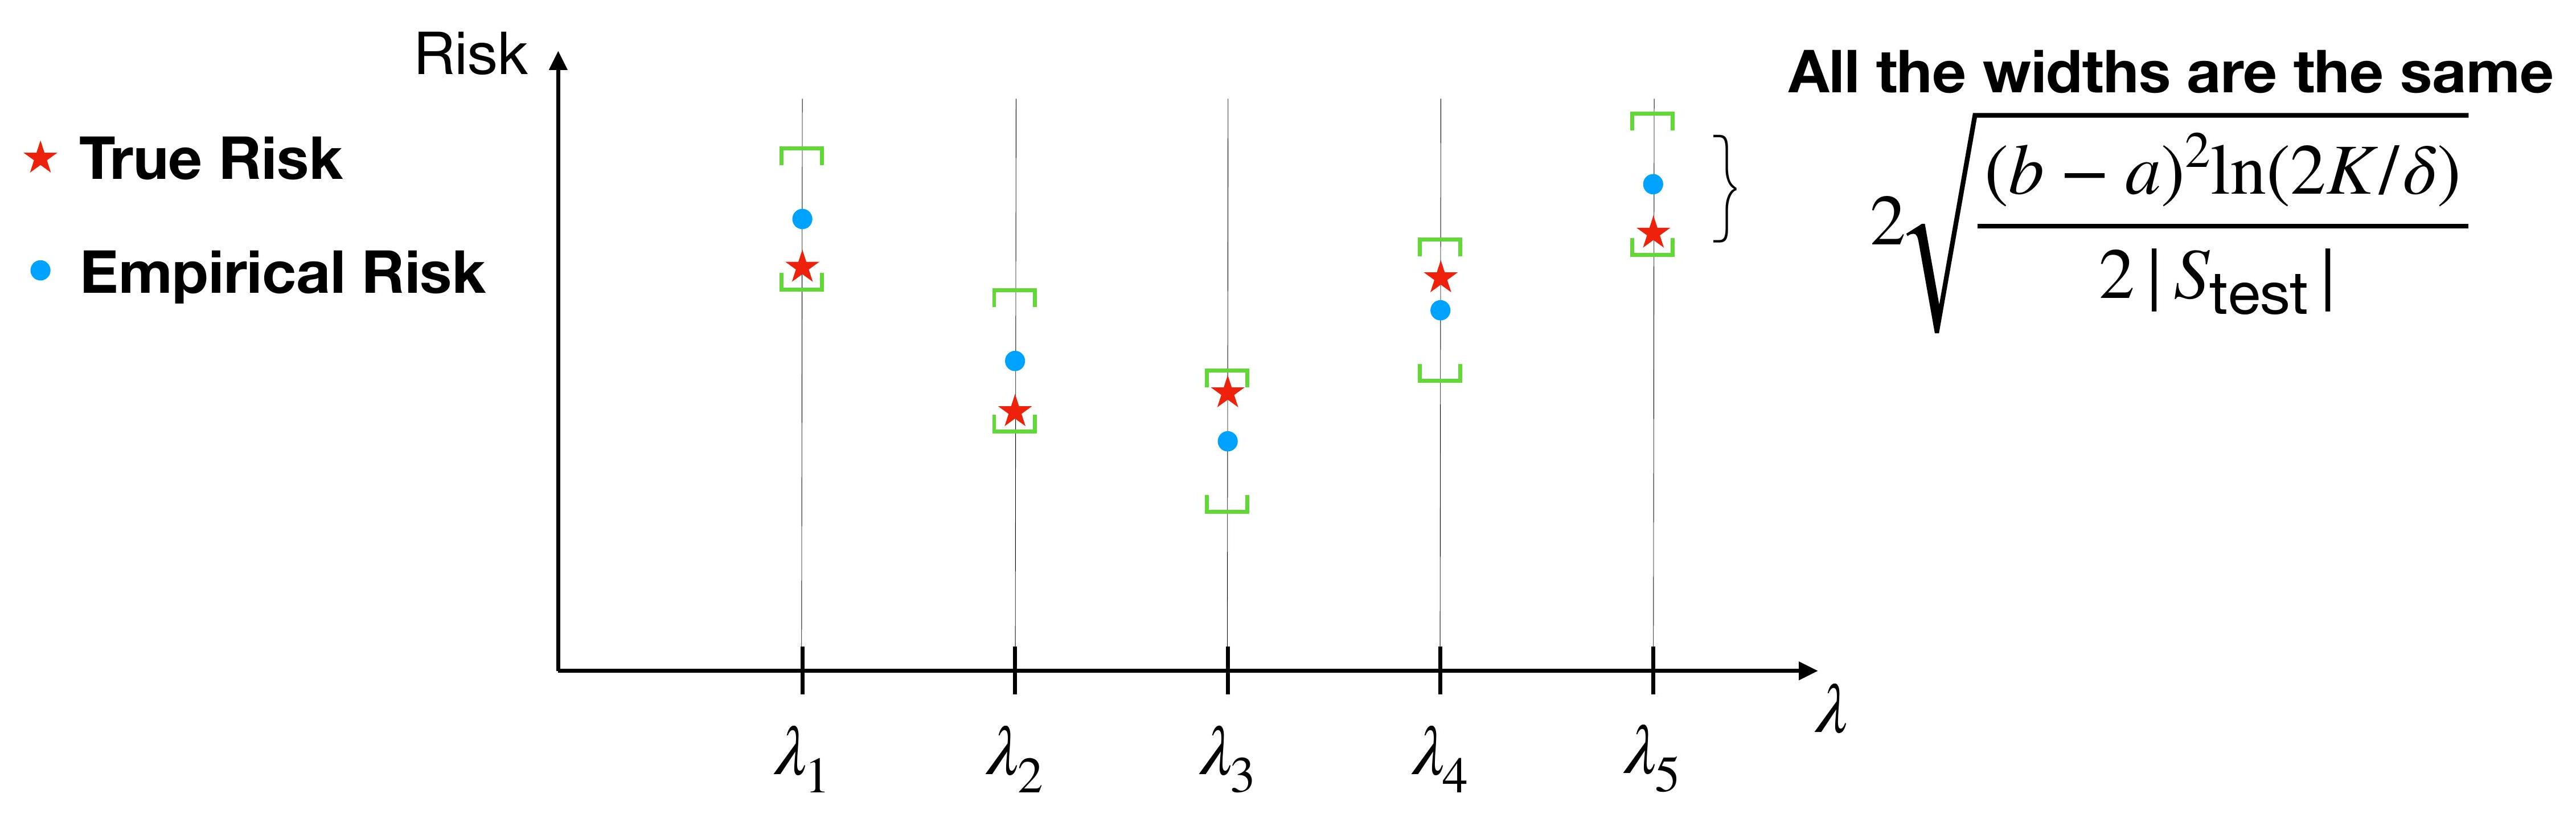
\includegraphics[max width=\textwidth]{2023_12_30_b4c98a1755bce7fa9493g-21}
\end{center}

Let $k^{*}=\operatorname{argmin}_{k} L_{\mathscr{D}}\left(f_{k}\right)$ and $\hat{k}=\operatorname{argmin}_{k} L_{S_{\text {test }}}\left(f_{k}\right)$ then

$$
\mathbb{P}\left[L_{\mathscr{D}}\left(f_{\hat{k}}\right) \geq L_{\mathscr{D}}\left(f_{k^{*}}\right)+2 \sqrt{\frac{(b-a)^{2} \ln (2 K / \delta)}{2\left|S_{\text {test }}\right|}}\right] \leq \delta
$$

Function with

Function with

the smallest empirical risk the smallest true risk

If we choose the "best" function according to the empirical risk then its true risk is not too far away from the true risk of the optimal choice

\begin{center}
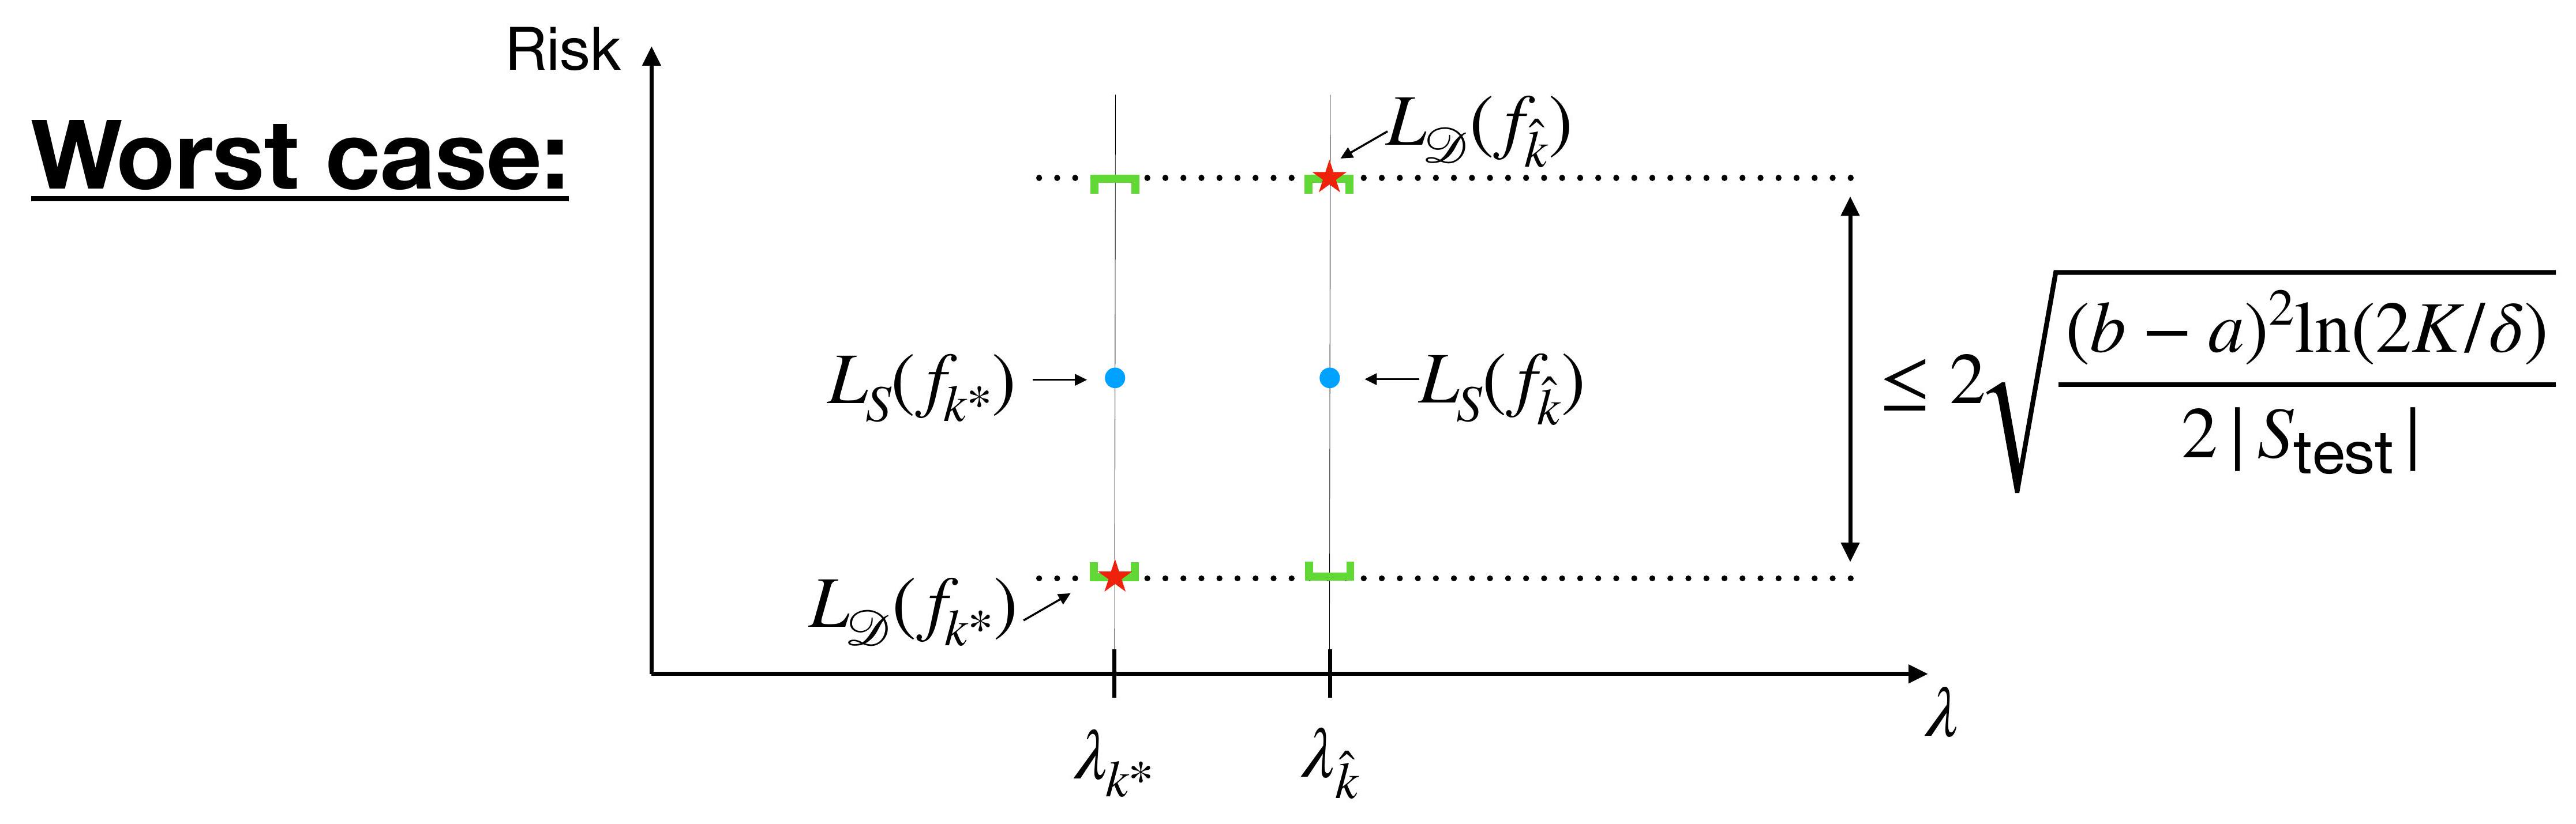
\includegraphics[max width=\textwidth]{2023_12_30_b4c98a1755bce7fa9493g-22}
\end{center}

Let $k^{*}=\operatorname{argmin}_{k} L_{\mathscr{D}}\left(f_{k}\right)$ and $\hat{k}=\operatorname{argmin}_{k} L_{S_{\text {test }}}\left(f_{k}\right)$ then

$$
\begin{aligned}
& \mathbb{P}\left[L_{\mathscr{D}}\left(f_{\hat{k}}\right) \geq L_{\mathscr{D}}\left(f_{k^{*}}\right)+2 \sqrt{\frac{(b-a)^{2} \ln (2 K / \delta)}{2\left|S_{\text {test }}\right|}}\right] \leq \delta \\
& \text { Function with } \\
& \text { Function with }
\end{aligned}
$$

\section*{Cross-Validation}
\begin{center}

\includegraphics[max width=\textwidth]{2023_12_30_b4c98a1755bce7fa9493g-23}
\end{center}

\begin{itemize}
  \item Splitting the data once into two parts (one for training and one for testing) is not the most efficient way to use the data
  \item Cross-validation is a better way
\end{itemize}

\section*{K-fold Cross-Validation}
\begin{enumerate}
  \item Randomly partition the data into $K$ groups
\end{enumerate}

\begin{center}

\includegraphics[max width=\textwidth]{2023_12_30_b4c98a1755bce7fa9493g-24}
\end{center}

run 1

\begin{center}

\includegraphics[max width=\textwidth]{2023_12_30_b4c98a1755bce7fa9493g-24(1)}
\end{center}

run 2 out exactly one of the $K$ groups for testing and use the remaining $K-1$ groups for training.

\begin{center}

\includegraphics[max width=\textwidth]{2023_12_30_b4c98a1755bce7fa9493g-24(3)}
\end{center}

run 3

\begin{center}

\includegraphics[max width=\textwidth]{2023_12_30_b4c98a1755bce7fa9493g-24(2)}
\end{center}

\begin{enumerate}
  \setcounter{enumi}{2}
  \item Average the $K$ results
\end{enumerate}

\begin{itemize}
  \item We have used all data for training, and all data for testing, and used each data point the same number of times
  \item Cross-validation returns an estimate of the generalization-error and its variance
\end{itemize}

\section*{Do we still have some time?}
Hoeffding's inequality:

Let $\Theta_{1}, \ldots, \Theta_{N}$ be a sequence of i.i.d. random variables with mean $\mathbb{E}[\Theta]$ and range $[a, b]$. Then, for any $\varepsilon>0$

$$
\mathbb{P}\left[\left|\frac{1}{N} \sum_{n=1}^{N} \Theta_{n}-\mathbb{E}[\Theta]\right| \geq \varepsilon\right] \leq 2 e^{-2 N \varepsilon^{2} /(b-a)^{2}}
$$

\section*{Proof (I)}
\begin{itemize}
  \item We equivalently assume that $\mathbb{E}[\Theta]=0$ and that $\Theta_{n} \in[a, b]$
  \item We will only show that
\end{itemize}

$$
\mathbb{P}\left\{\frac{1}{N} \sum_{n=1}^{N} \Theta_{n} \geq \varepsilon\right\} \leq e^{-2 N \varepsilon^{2} /(b-a)^{2}}
$$

This, together with the equivalent bound

$$
\mathbb{P}\left\{\frac{1}{N} \sum_{n=1}^{N} \Theta_{n} \leq-\varepsilon\right\} \leq e^{-2 N \varepsilon^{2} /(b-a)^{2}}
$$

will prove the claim

\section*{Proof (II)}
For any $s \geq 0, \quad \mathbb{P}\left\{\frac{1}{N} \sum_{n=1}^{N} \Theta_{n} \geq \varepsilon\right\}=\mathbb{P}\left\{s \frac{1}{N} \sum_{n=1}^{N} \Theta_{n} \geq s \varepsilon\right\}$

$$
=\mathbb{P}\left\{e^{s \frac{1}{N} \sum_{n=1}^{N} \Theta_{n}} \geq e^{s \varepsilon}\right\}
$$

$$
\begin{aligned}
& \leq \mathbb{E}\left[e^{s \frac{1}{N} \sum_{n=1}^{N} \Theta_{n}}\right] e^{-s \varepsilon} \quad \text { (Markov inequality) } \\
& =\prod_{n=1}^{N} \mathbb{E}\left[e^{\frac{s \Theta_{n}}{N}}\right] e^{-s \varepsilon} \quad \text { (the r.v } \Theta_{n} \text { are independent) } \\
& =\mathbb{E}\left[e^{\frac{s \Theta}{N}}\right]^{N} e^{-s \varepsilon} \quad \quad \text { (the r.v } \Theta_{n} \text { are i.d.) } \\
& \leq e^{s^{2}(b-a)^{2} /(8 N)} e^{-s \varepsilon} \quad \text { (Hoeffding lemma) }
\end{aligned}
$$

\section*{Proof (III)}
What do we do now? We have for any $s \geq 0$

$$
\mathbb{P}\left\{\frac{1}{N} \sum_{n=1}^{N} \Theta_{n} \geq \varepsilon\right\} \leq e^{s^{2}(b-a)^{2} /(8 N)} e^{-s \varepsilon}
$$

In particular for the minimum value obtained for $s=\frac{4 N \varepsilon}{(b-a)^{2}}$

$$
\mathbb{P}\left\{\frac{1}{N} \sum_{n=1}^{N} \Theta_{n} \geq \varepsilon\right\} \leq e^{-2 N \varepsilon^{2} /(b-a)^{2}}
$$

\section*{Hoeffding lemma}
For any random variable $X$, with $\mathbb{E}[X]=0$ and $X \in[a, b]$ we have

$$
\mathbb{E}\left[e^{s X}\right] \leq e^{\frac{1}{8} s^{2}(b-a)^{2}} \text { for any } s \geq 0
$$

Proof outline:

Consider the convex function $s \mapsto e^{s x}$. In the range $[a, b]$ it is upper bounded by the chord

$$
e^{s x} \leq \frac{x-a}{b-a} e^{s b}+\frac{b-x}{b-a} e^{s a}
$$

Taking the expectation and recalling that $\mathbb{E}[X]=0$, we get

$$
\mathbb{E}\left[e^{s X}\right] \leq \frac{b}{b-a} e^{s a}-\frac{a}{b-a} e^{s b} \leq e^{s^{2}(b-a)^{2} / 8}
$$


\end{document}